

Cloud computing\cite{mell2011nist} is a technology that is becoming extensively popular and usually is referred to being massively scalable. This is primarily due to the fact of cloud computing's elastic nature. Elasticity in cloud is generally referred for the usage of cloud resources on-demand\cite{mell2011nist}, and pay only for the resources being used. The resources provisioning are usually in the form of virtual machines (VM). Provisioning of VM is made possible through distributed, large-scale computing clusters, often driven by server virtualization software, like VMware ESX Server\cite{vmwareesx}, Xen\cite{xenhyper} or KVM\cite{kvmhyper}. Organizations which use or migrate to cloud, use cloud for different purposes such as running batch jobs, hosting web application or for storage and backup.
\\
cloud hosted applications are likely to deliver high quality of service (QoS). The workload of an hosted application varies according to the time of the day and rises sharply on certain trends. For example, an online retailer faces spikes of workload on a new launch of smartphone and a daily cyclical workload variations\cite{dawoud2013scalability}. On the other hand, a video on demand provider anticipate peak workload on a video going viral\cite{niu2012quality}. However, the cloud infrastructure provides an elastic environment for these applications to scale up and down according to workload variations.

\section{Motivation}
\label{sec:Motivation}
Cloud computing architecture enables an application to cope with rapidly varying workloads. Timely provisioning VMs in the cloud implies an overhead. The overhead can lead to period of over-utilization of the VMs which degrades the QoS. Moreover, due to workload consolidation in cloud infrastructures, the performance of an application can be influenced by other co-located VM's. Few of the several challenges faced while managing the performance of an application while maintaining high QoS are listed below:
\begin{itemize}
  \item \textbf{Resource Acquisition} The overhead of provisioning a right VM instance type and right number of VM instances in public or private cloud is a problem. The overhead is attributed to the IaaS cloud vendors, such as Amazon EC2\cite{amazon2010amazon}, Rackspace\cite{rackspace2010inc},etc., apply diverse VM instance pricing models at different commitment levels. At one level, cloud users launch on-demand instances and pay only for instance-hours, without making any long-term upfront commitments. At the other level, there are reserved instances wherein users prepay a one-time/partial upfront fee and then reserve an instance either for 1-year or 3-years, where in the instance prices have a significant discount. Table~\ref{table:cost}\footnote{Latest price from : \url{https://aws.amazon.com/ec2/pricing/}} gives a pricing example of on-demand and reserved instances in Amazon EC2.
  \item \textbf{VM Start \& Shutdown Time} Scalability in cloud involves acquiring and release of resources based on application workloads\cite{roy2011efficient}. Task of scaling the resources in cloud require programming against cloud service provider API's. Acquiring and releasing of resources incur performance overhead steaming in: API request, communication overhead, scheduling delay, VM startup time, application startup time and update of application state if any\cite{roy2011efficient}. Mao \& Humphrey\cite{mao2012performance} has studied VM startup time in various cloud services provider like Amazon AWS, Microsoft Azure, and Rackspace. The startup time of various VM instances are showed in the Figure~\ref{figure:vmstartuptimes} . The Table~\ref{table:avgvmtime} shows the average startup times for various VM instance types. For example, on Amazon AWS average Windows startup time is 810.2 seconds. This long unpredictable VM startup time make it hard in resource acquisition and making it available for the applications. This leads to another problem of understanding VM startup and shutdown times, to help cloud hosted applications to plan ahead and make resource available on time.
  \item \textbf{Forecasting Future Workloads} Due to the above mentioned VM Start and Shutdown time delays, it is desirable to acquire VM's needed before hand than acquiring the resources just-in-time when workload increases\cite{roy2011efficient}. This can be possibly solved by predicting future workloads, by developing a forecast model from historical data\cite{roy2011efficient}.
  \item \textbf{QoS \& Rapid Workload Changes} The workload of a cloud hosted application varies dynamically over multiple period of time. A period of sudden increase in workload can lead to over-utilization of VM's. During overload periods the QoS may degrade to a very low levels or may have total denial of service. In production environments, such behavior is harmful for the reputation of the application providers. For example, consider Figure~\ref{figure:sampleworkload} which depicts a real-world workload trace of user request to Audio conferencing application from Citrix Inc. VM provisioning for such a system is not easy. VM's can be provisioned for the average load or for the peak load periods. Each approach has its disadvantages. When planning with average load, there is less cost incurred due to less number of VM's provisioned, but VM's will be over-utilized under peak load hence violating SLA. Whereas, planning for peak load will lead to VM's being under utilized or idle in non peak load and hence incurring high cost.
\end{itemize}

\begin{figure}[h]
  \begin{center}
    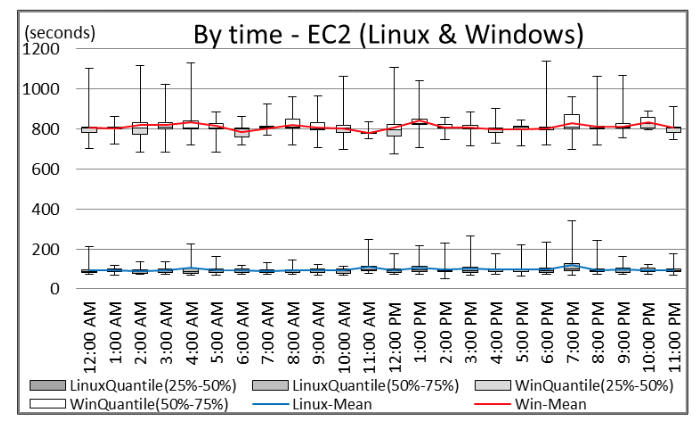
\includegraphics[scale=0.8]{vmstarttimes.png}
    \caption{EC2 VM startup time by time of the day (From\cite{mao2012performance})}
    \label{figure:vmstartuptimes}
  \end{center}
\end{figure}

\begin{flushleft}
  \begin{table}
    \begin{tabular}{ | l | l | l |}
      \hline
      Cloud & OS & Average VM startup time (in Seconds) \\ \hline
      EC2 & Linux & 96.9 \\ \hline
      EC2 & Windows & 810.2 \\ \hline
      Azure & WebRole & 374.8 \\ \hline
      Azure & WorkerRole & 406.2 \\ \hline
      Azure & VMRole & 356.6 \\ \hline
      Rackspace & Linux & 44.2 \\ \hline
      Rackspace & Windows & 429.2 \\ \hline
    \end{tabular}
    \caption{Average VM startup times (From\cite{mao2012performance})}
     \label{table:avgvmtime}
\end{table}
\end{flushleft}

Acquiring instances at the cost-optimal commitment level plays a central role for QoS versus cost management. This drives the motivation to build an efficient and flexible algorithm for provisioning and managing the VM instances.
\begin{flushleft}
  \begin{table}
    \begin{tabular}{ | L{2cm} | L{2cm} | L{2cm} | L{2cm} | L{2cm} | L{2cm} |}
      \hline
      Name & Upfrom Cost & Effective hourly cost & Effective montly cost & 1 year cost & 3 year cost \\ \hline
      On-demand & --- & 0.95 & 613.42 & 7361.04 & 22083.12 \\ \hline
      1-year reserved No upfront & 0.0 & 0.65 & 453.33 & 5439.96 & 16319.88 \\ \hline
      1-year reserved partial upfront & 2361.0 & 0.537 & 391.66 & 4699.92 & 14099.76 \\ \hline
      3-year reserved full upfront & 8580.0 & 0.327 & 238.34 & --- & 8580.0 \\ \hline
    \end{tabular}
    \caption{Instance Pricing Option for c4.4xlarge Linux instance type (prices in USD)}
     \label{table:cost}
\end{table}
\end{flushleft}

\begin{figure}[h]
  \begin{center}
    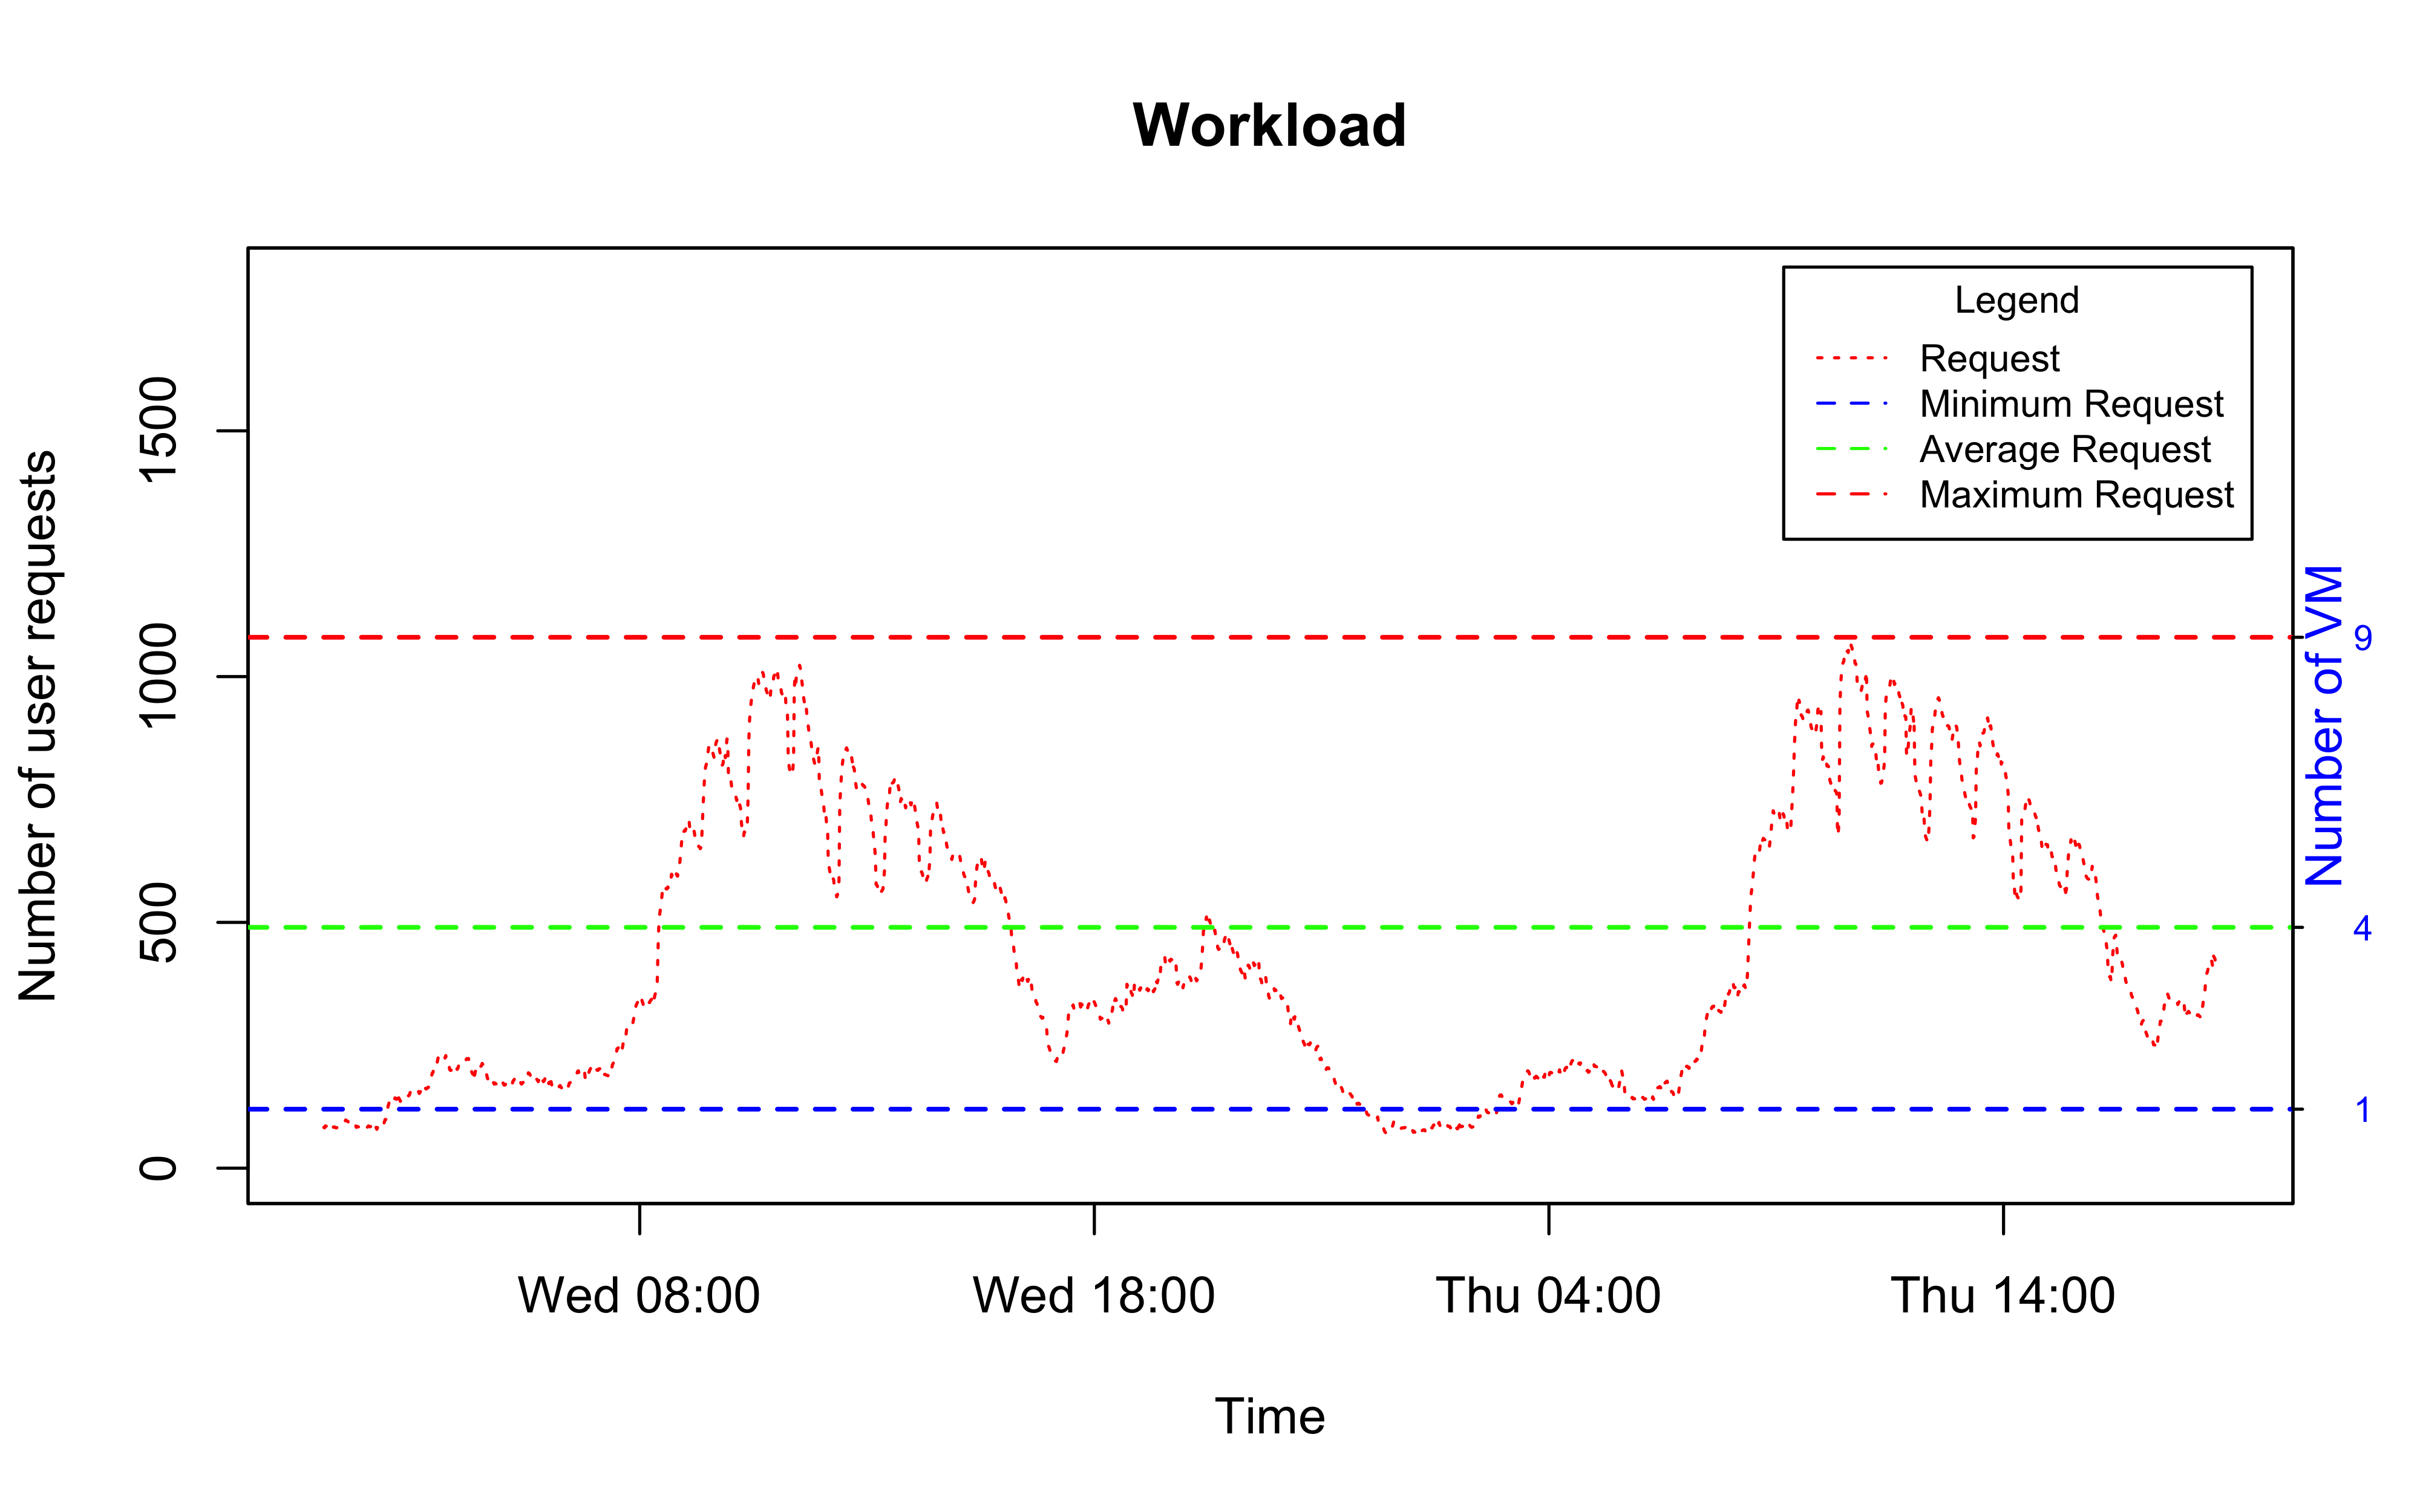
\includegraphics[scale=0.1]{workloadforsim}
    \caption{Sample Workload}
    \label{figure:sampleworkload}
  \end{center}
\end{figure}


\section{Research Questions}

\label{sec:Research Questions}

Due to the challenges stated in the Section~\ref{sec:Motivation}, the goal of this thesis work is to design and implement an algorithm which can:

\begin{itemize}
  \item Compute the right number of VM resources required for the expected increase or decrease in workload.
  \item Ability to satisfies both application QoS and low operational cost by using different instance types provided by cloud service providers.
  \item Forecast future workload to proactively provision VM's to mitigate effects of delay in VM start and shutdown time overhead.
\end{itemize}

Based on this goal, four main research questions can be addressed and shall be answered within this thesis:

\begin{enumerate}
  \item What are the parameters to consider while computing the right number of VM resources required to satisfies QoS guaranties?
  \item What are the right VM instance types to use to achieve low operational cost?
  \item What kind of tool and technique can be used to accurately evaluate the performance and cost of the scaling algorithm without actual deployment on the clouds?
  \item What are the forecasting techniques which can be used to proactively provision VM's to mitigate effects of delay in VM start and shutdown time?
\end{enumerate}

\section{Contributions}
\label{sec:Contributions}
This thesis address the challenges mentioned in Section~\ref{sec:Motivation} with customer-oriented solution. At the beginning of this thesis, the state of the art techniques in customer-oriented solutions that do not employ cloud service provider involvement in the automated scaling of an application is investigated. On the light of these requirement, an proactive optimized threshold based\cite{lorido2012auto} automated scaling algorithm, named AppElastic, is proposed. AppElastic algorithm deals with the horizontal scalability\cite{vaquero2011dynamically} in IaaS mode. It address the trade-off problem between cost and QoS guaranties by employing very popular threshold based rules automated scaling algorithm. AppElastic employs time series forecasting to proactively compute the number of VM's needed to satisfy the QoS guaranties of the application. In this thesis the trade-off between the QoS and the cost is considered. Finally, to avoid the impact from arbitrary workload, AppElastic algorithm is designed to terminate the VM's which are nearing instance-hour.
\\
An experimental study on the performance evaluation of AppElastic algorithm at large-scale, a simulation based mode, called ElasticSim, is developed. ElasticSim evaluates the cost and performance of public IaaS clouds along with VM instances and diverse workload patterns. ElasticSim is fed with workload trace from Citrix audio/video conferencing application. The results show that optimizing the scalability thresholds and adopting proactive scalability can mitigate the resource provisioning overhead with cost benefits.




% remove this before sending it for the review.
%\bibliography{../handin}
